\documentclass[
%% TIKZ_CLASSOPTION %%
tikz
]{standalone}
\usepackage{amsmath}
\usetikzlibrary{matrix}
%% EXTRA_TIKZ_PREAMBLE_CODE %%
\begin{document}
%% TIKZ_CODE %%
\usetikzlibrary{shapes,decorations,arrows,calc,arrows.meta,fit,positioning}
\tikzset{
    -Latex,auto,node distance =1 cm and 1 cm,semithick,
    state/.style ={ellipse, draw, minimum width = 0.7 cm},
    point/.style = {circle, draw, inner sep=0.04cm,fill,node contents={}},
    bidirected/.style={Latex-Latex,dashed},
    el/.style = {inner sep=2pt, align=left, sloped}
}
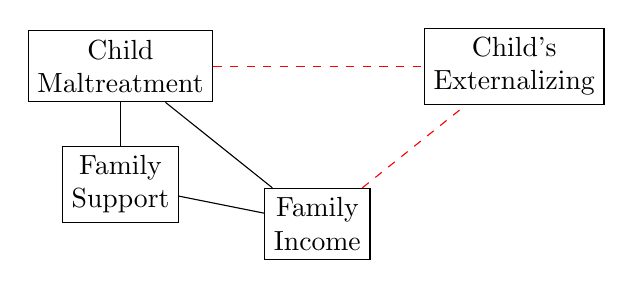
\begin{tikzpicture}
    \node[draw, align=center] (1) at (0,0) {Child\\Maltreatment};
    \node[draw, align=center] (2) at (5,0) {Child's\\Externalizing};
    \node[draw, align=center] (3) at (2.5,-2) {Family\\Income};
    \node[draw, align=center] (4) at (0,-1.5) {Family\\Support};
    \path[dashed,red] (1) edge  (2);
    \path (3) edge (1);
    \path[dashed,red] (3) edge (2);
    \path (4) edge (1);
    \path (3) edge (4);
\end{tikzpicture}
\end{document}
